\chapter{An Autonomous AI Agent for Benchmark Campaigns}
\label{chap:benchmark-agent}

\section*{Introduction}

The previous chapter presented a tool that analyses the \emph{output} of a benchmark ---
two linker maps produced by completed builds. However, producing those builds in the first
place is itself a substantial engineering task. Each new cross-vendor comparison requires
creating a benchmark project for the competitor platform, porting the STM32 reference code
while preserving its exact runtime semantics, configuring the IAR Embedded Workbench for
ARM (EWARM) project correctly, and debugging the inevitable compiler, linker, and runtime
issues that arise when targeting unfamiliar silicon. Done manually, this process is slow,
error-prone, and difficult to keep consistent across many vendor comparisons.

To address this, we designed and built the \emph{MCU Benchmark Copilot Agent} --- a custom
GitHub Copilot agent system that operates inside Visual Studio Code (VS Code) and
\emph{autonomously} drives end-to-end benchmark campaigns: from scenario resolution and
firmware acquisition, through project creation, IAR build automation, evidence-driven
debugging, measurement extraction, and semantic-equivalence verification~\cite{vscode,
github-copilot}. Unlike a passive assistant, the agent executes builds, fetches missing
materials from official vendor sources, applies fixes, and iterates --- asking the user
only before programming physical hardware. Where MCU Workflow Studio analyses what
\emph{exists}, the agent system \emph{creates} what does not yet exist, and it does so
under strict rules that enforce semantic equivalence and benchmark fairness at every step.
The two tools are complementary: the agent produces validated builds, and the studio
analyses their footprint.

This chapter documents the agent as an engineering contribution. We describe the problem it
addresses, its layered architecture (agents, skills, automation tools, configuration
registry), its deterministic campaign workflow, the always-on policies that govern its
behaviour, and its integration with the broader benchmarking effort.

\section{The benchmark engineering problem}
\label{sec:agent-problem}

A single STM32-versus-competitor benchmark involves several non-trivial steps. The STM32
reference project must first be understood in full --- task structure, timing, peripheral
usage, reporting format, and observable behaviour. A corresponding project must then be
created for the target platform, mapping every STM32 hardware abstraction layer (HAL) call
to the competitor's equivalent application programming interface (API) without altering the
benchmark's semantics. The resulting project must be configured for the IAR
toolchain~\cite{iar-ewarm} with the correct device selection, startup file, linker
configuration, include paths, and compiler defines. Once it compiles, runtime issues --- wrong interrupt vectors,
misconfigured clocks, broken universal asynchronous receiver-transmitter (UART) output ---
must be diagnosed from real evidence rather than guesswork. And throughout, the comparison
must remain fair: same optimisation level, same measurement scope, same observable output
format.

Doing this for one vendor pair and one software stack is manageable. Repeating it for
multiple vendors (GigaDevice, NXP, Renesas, Texas Instruments, Infineon, Nordic,
Microchip) across multiple stacks (USB device, FreeRTOS, CoreMark) quickly becomes the
dominant time cost of the benchmarking campaign. Each port also carries a risk of
\emph{semantic drift} --- subtle changes in task priorities, timing, or synchronisation
that invalidate the comparison without being immediately visible.

We needed a system that could enforce the methodology consistently across every port,
refuse to guess when evidence was missing, execute deterministic build and measurement
workflows without manual intervention, and make its reasoning transparent. A
general-purpose large language model (LLM) cannot do this out of the box: it lacks the
domain-specific checklists, the structured routing, the automation tooling, and the policy
of refusing to claim success without hardware evidence. A custom agent system, built on VS
Code's Copilot extensibility framework, gave us the ability to encode our benchmarking
methodology --- and to \emph{execute} it autonomously --- directly within the development
environment~\cite{vscode-agent-mode}.

\section{Architecture}
\label{sec:agent-architecture}

The system is structured as four cooperating layers: specialist \emph{agents} that handle
reasoning and delegation, reusable \emph{skills} that encode methodology as checklists,
\emph{automation tools} (PowerShell and Python scripts) that perform deterministic
operations, and a \emph{configuration registry} (YAML files) that provides ground truth
about boards, MCUs, vendors, toolchains, and measurement profiles. A shared set of
always-on rules governs all layers. All configuration lives in a \texttt{.github/}
directory within the benchmark workspace --- no compiled code, no external server, no
deployment step. The agents run inside VS Code's GitHub Copilot Chat
extension~\cite{github-copilot} and have access to the workspace file system, terminal,
web, and search capabilities.

Figure~\ref{fig:agent-architecture} illustrates the layered arrangement. A user request
enters the coordinator agent, which resolves the scenario, classifies the task, acquires
missing materials, and delegates to the appropriate specialist agent or invokes a skill
workflow. Specialist agents operate in isolated context, use the automation tools for
deterministic operations, and return structured results.

\begin{figure}[H]
\centering
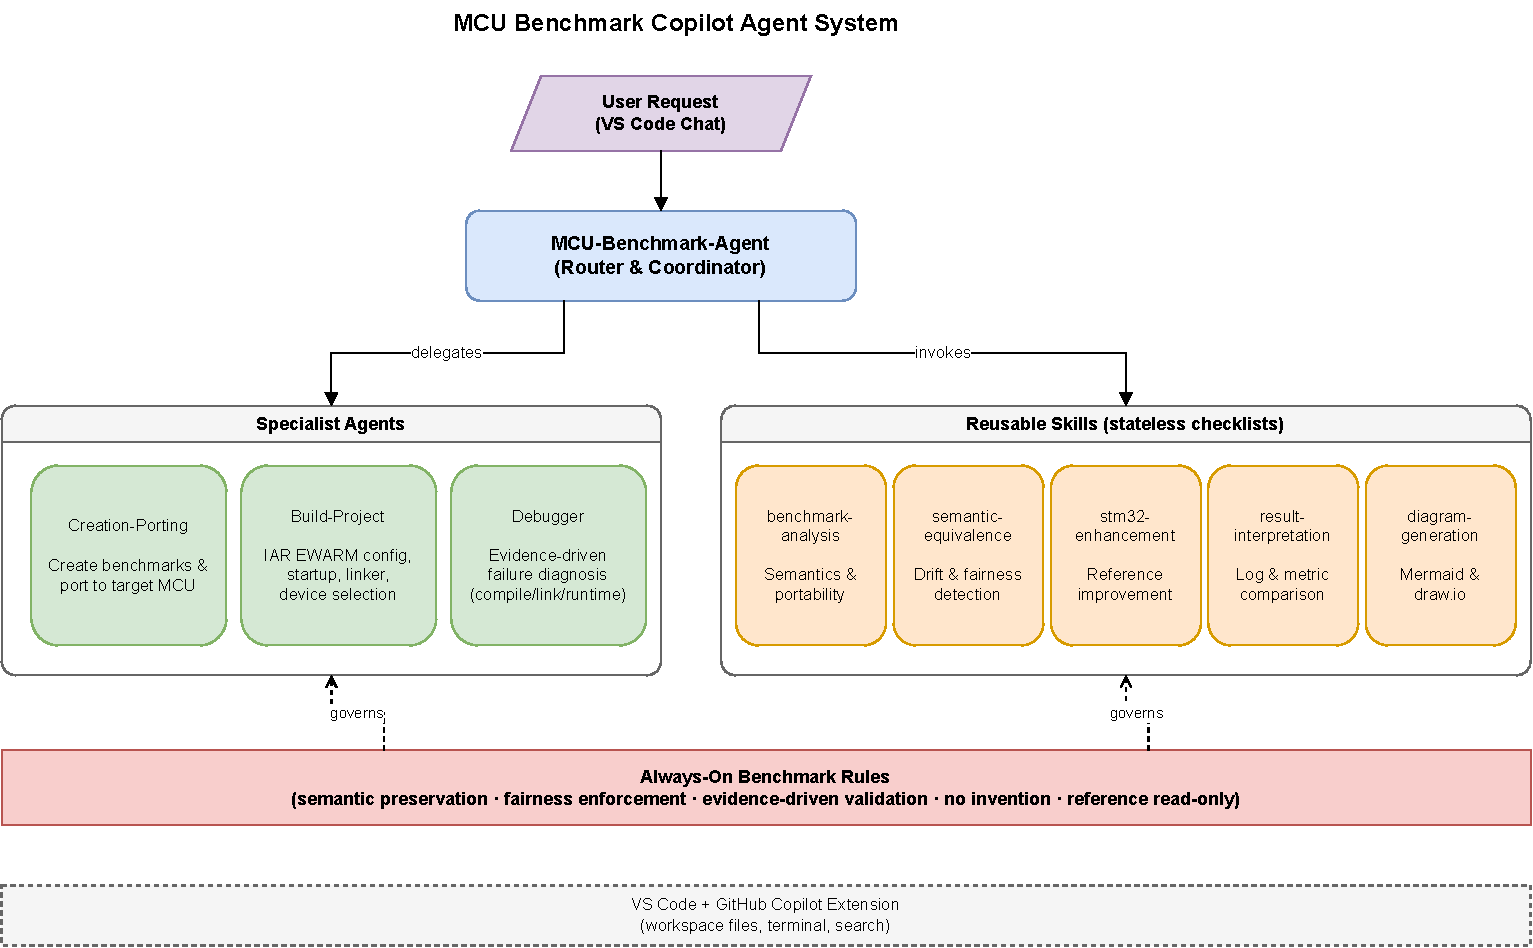
\includegraphics[width=\textwidth]{Figures/benchmark-agent/architecture.pdf}
\caption{Architecture of the MCU Benchmark Copilot Agent system. The coordinator resolves
scenarios and delegates to specialist agents; automation tools handle deterministic
build/measurement operations; all layers operate under the shared always-on benchmark rules
and consult the configuration registry.}
\label{fig:agent-architecture}
\end{figure}

\subsection{The four specialist agents}
\label{sec:agent-specialists}

Each agent has a defined responsibility, a restricted tool set, an autonomy contract, and a
structured output contract. Table~\ref{tab:agent-roles} summarises them.

\begin{table}[H]
\centering
\caption{Specialist agents and their responsibilities.}
\label{tab:agent-roles}
\begin{tabularx}{\textwidth}{l l X}
\toprule
\textbf{Agent} & \textbf{Role} & \textbf{Responsibility} \\
\midrule
MCU-Benchmark-Agent & Autonomous coordinator & Resolves scenarios from partial input, acquires missing materials, orchestrates end-to-end campaigns, delegates to specialists. Full tool access including web and execute. \\
Creation-Porting & Project generation & Creates new benchmark projects from scratch or ports existing benchmarks in any direction (STM32$\to$competitor, competitor$\to$STM32, vendor$\to$vendor, board$\to$board). Acquires firmware autonomously. \\
Build-Project & Build automation & Autonomously executes IAR builds, classifies failures, applies project-level fixes, and rebuilds --- without user intervention for non-hardware tasks. \\
Debugger & Failure diagnosis & Autonomously diagnoses compiler, linker, and runtime failures; extracts measurements from logs and captures; applies minimal fixes and revalidates. \\
\bottomrule
\end{tabularx}
\end{table}

The coordinator's routing decision tree is deterministic: project understanding goes to the
\emph{benchmark-analysis} skill; cross-vendor porting goes to \emph{Creation-Porting};
build execution and configuration go to \emph{Build-Project}; failures accompanied by real
evidence go to \emph{Debugger}; and result interpretation uses the dedicated skill. This
routing prevents a general-purpose model from attempting tasks outside its configured
expertise and ensures each specialist receives only the context it needs.

Figure~\ref{fig:agent-use-case} presents a complete use case diagram of the system,
showing all actors, the twenty internal capabilities, and the hardware approval boundary
that separates autonomous operations from those requiring user confirmation.

\begin{figure}[H]
\centering
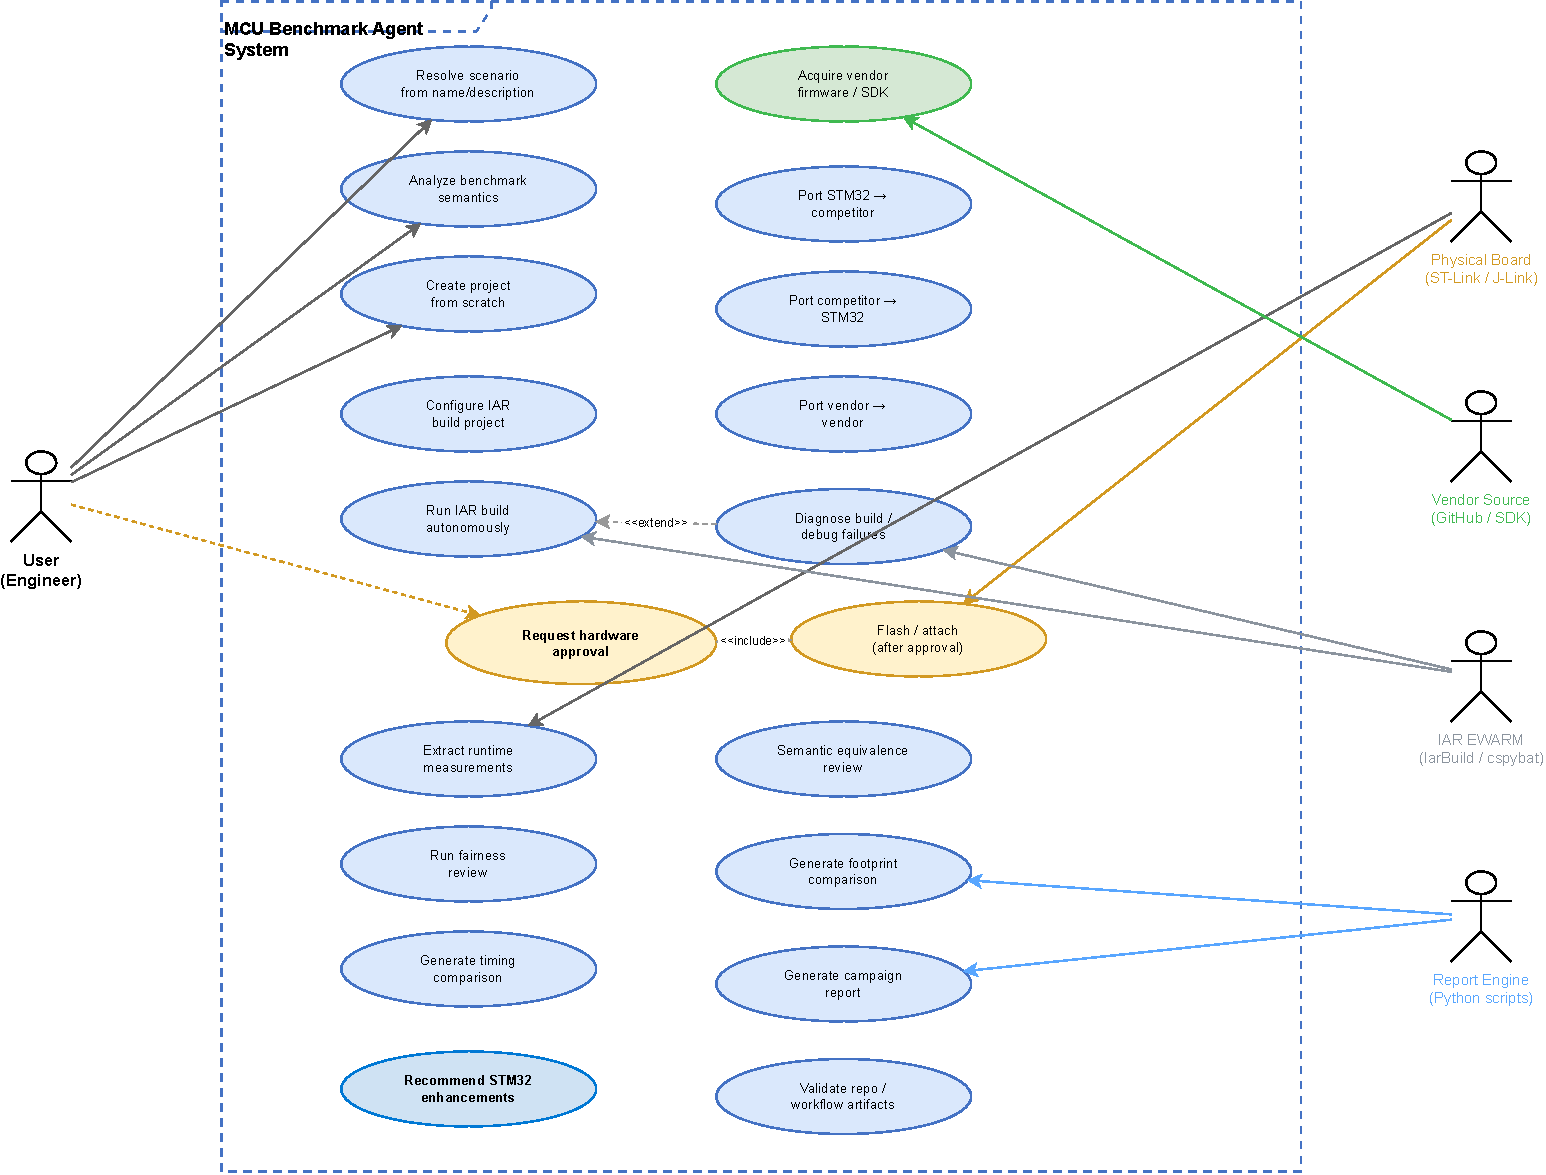
\includegraphics[width=\textwidth]{Figures/benchmark-agent/use-case.pdf}
\caption{UML use case diagram of the MCU Benchmark Copilot Agent system. Blue ellipses
represent autonomous use cases; yellow ellipses require user approval; green indicates
external acquisition. External actors include the user, physical board, vendor source
repositories, IAR EWARM toolchain, and the report engine scripts.}
\label{fig:agent-use-case}
\end{figure}

\subsection{The six reusable skills}
\label{sec:agent-skills}

Skills encode repeatable workflows as structured Markdown checklists. Unlike agents, they
do not receive isolated context or delegated reasoning --- they provide structure, not
autonomy. Table~\ref{tab:agent-skills} lists them.

\begin{table}[H]
\centering
\caption{Reusable skills and their purposes.}
\label{tab:agent-skills}
\begin{tabularx}{\textwidth}{l X l}
\toprule
\textbf{Skill} & \textbf{Purpose} & \textbf{Primary users} \\
\midrule
benchmark-analysis & File classification, semantics extraction, and portability split of an existing project. & Coordinator, Creation-Porting \\
semantic-equivalence & Reference-versus-target behaviour comparison and drift detection. & Coordinator, Creation-Porting \\
iar-template-resolution & Resolve, acquire, and integrate IAR project templates per board type using a deterministic lookup algorithm. & Creation-Porting, Build-Project \\
stm32-enhancement & Gap-driven recommendations for improving STM32 reference portability. & Coordinator \\
result-interpretation & Comparative interpretation of benchmark logs, measurements, and result files. & Coordinator, Debugger \\
diagram-generation & Mermaid and draw.io workflow, architecture, and presentation diagrams. & Coordinator \\
\bottomrule
\end{tabularx}
\end{table}

\subsection{Automation tools}
\label{sec:agent-tools}

A critical addition to the system is a library of twelve deterministic scripts
(\texttt{.github/tools/}) that the agents invoke via the terminal for operations that must
produce repeatable results. Table~\ref{tab:agent-automation-tools} lists the key scripts.

\begin{table}[H]
\centering
\caption{Automation tools in the agent system.}
\label{tab:agent-automation-tools}
\begin{tabularx}{\textwidth}{l l X}
\toprule
\textbf{Script} & \textbf{Language} & \textbf{Purpose} \\
\midrule
\texttt{run\_iar\_build.ps1} & PowerShell & Wraps IarBuild.exe with structured output, exit-code handling, and log capture. \\
\texttt{discover\_iar.ps1} & PowerShell & Deterministic IAR installation discovery at known paths. \\
\texttt{acquire\_iar\_template.ps1} & PowerShell & Downloads and materialises IAR board templates from official vendor sources. \\
\texttt{run\_cspy\_capture.ps1} & PowerShell & Runs cspybat.exe batch debug sessions and captures measurement output~\cite{iar-cspybat}. \\
\texttt{collect\_measurements.py} & Python & Parses UART, SWO, and C-SPY output into structured measurement YAML. \\
\texttt{normalize\_measurements.py} & Python & Normalises raw measurements for cross-platform comparison. \\
\texttt{compare\_measurements.py} & Python & Computes deltas and fairness-aware comparisons between platforms. \\
\texttt{normalize\_build\_log.py} & Python & Structures IAR build diagnostics into classified error/warning lists. \\
\texttt{parse\_map\_file.py} & Python & Extracts memory-usage data from IAR linker map files. \\
\texttt{generate\_benchmark\_report.py} & Python & Produces structured campaign reports from collected artifacts. \\
\texttt{validate\_benchmark\_repo.py} & Python & Validates workspace structure and campaign artifact completeness. \\
\texttt{validate\_iar\_templates.py} & Python & Checks materialized IAR templates against expected file inventories. \\
\bottomrule
\end{tabularx}
\end{table}

These scripts ensure that build commands, measurement parsing, and comparison logic execute
identically regardless of which agent invokes them or when. The agents handle reasoning and
decision-making; the scripts handle deterministic execution.

\subsection{Configuration registry}
\label{sec:agent-config-registry}

The YAML-based configuration registry (\texttt{.github/config/}) provides ground truth
that the agents consult rather than hallucinate. Table~\ref{tab:agent-config-files} lists
its files.

\begin{table}[H]
\centering
\caption{Configuration registry files.}
\label{tab:agent-config-files}
\begin{tabularx}{\textwidth}{l X}
\toprule
\textbf{File} & \textbf{Content} \\
\midrule
\texttt{boards.yaml} & Board registry with official identifiers, MCU, core, probe, measurement capabilities, and aliases for all supported evaluation boards. \\
\texttt{mcus.yaml} & MCU specifications: flash, RAM, clock, peripherals, startup and linker file references. \\
\texttt{vendors.yaml} & Vendor metadata: supported families, HAL framework, RTOS defaults, wrapper model, and board naming conventions for ST, TI, NXP, Renesas, GigaDevice, Infineon, Nordic, and Microchip. \\
\texttt{toolchains.yaml} & IAR EWARM binary paths, discovery order, build-command patterns, and configuration areas. \\
\texttt{iar\_templates.yaml} & IAR project template registry with acquisition status, source URLs, and resolution algorithm metadata. \\
\texttt{vendor\_sources.yaml} & Official firmware acquisition URLs and SDK references per vendor. \\
\texttt{measurement\_profiles.yaml} & Standard measurement definitions (task-switch cycles, IRQ latency, flash/RAM footprint) with fairness risks and required evidence. \\
\texttt{reporting.yaml} & Output format templates for campaign reports. \\
\bottomrule
\end{tabularx}
\end{table}

The registry solves a fundamental problem with LLM-based agents: when the model does not
know a board's pin mapping or a vendor's SDK repository URL, it might invent one. By
encoding verified facts in YAML and instructing the agents to consult these files, we
eliminate an entire class of hallucination errors.

\section{Supported workflow directions}
\label{sec:agent-directions}

A key design decision was to support benchmarking in \emph{all} directions, not only the
obvious STM32-to-competitor port. The system handles six workflow directions:

\begin{enumerate}
\item \textbf{STM32 $\to$ competitor} --- port an STM32 reference benchmark to a competitor target (the primary use case).
\item \textbf{Competitor $\to$ STM32} --- port a competitor's reference project to an STM32 target (useful when the competitor has a ready example that ST lacks).
\item \textbf{Vendor~A $\to$ Vendor~B} --- port between any two non-ST vendors.
\item \textbf{Board~A $\to$ Board~B} --- replicate a ready scenario on a different board (same or different vendor).
\item \textbf{Scenario description $\to$ new project from scratch} --- create a complete benchmark project from only a textual scenario description, with no pre-existing reference code.
\item \textbf{Firmware/benchmark name only $\to$ acquire and build} --- the user provides only a firmware package name (e.g.\ \texttt{USB\_Device\_HID}); the agent resolves the scenario, acquires the firmware from official sources, and proceeds autonomously.
\end{enumerate}

In all directions, the same semantic preservation and fairness rules apply. The agent
generates a new target project rather than modifying any reference, and it preserves
benchmark semantics (observable behaviours), not vendor API names.

\section{Autonomy model and approval gates}
\label{sec:agent-autonomy}

The agent operates autonomously by default for all workspace inspection, file generation,
build execution, debug preparation, material acquisition, and measurement extraction.
Table~\ref{tab:agent-autonomy} clarifies the boundary.

\begin{table}[H]
\centering
\caption{Autonomy model: autonomous actions versus approval-required actions.}
\label{tab:agent-autonomy}
\begin{tabularx}{\textwidth}{X X}
\toprule
\textbf{Autonomous (no confirmation)} & \textbf{Requires user approval} \\
\midrule
Read, search, and inspect any workspace file &
Flash or program a physical board \\

Create, edit, or reorganise application-layer project files &
Erase or reset a physical device \\

Run IarBuild.exe and other local build commands &
Attach a live debug probe to real hardware \\

Parse build logs, linker maps, UART output, and debugger captures &
Modify vendor baseline file contents (startup, linker, HAL, BSP, middleware) \\

Fetch firmware, CMSIS headers, BSP, and documentation from official vendor sources &
--- \\

Apply minimal project-configuration fixes and rebuild &
--- \\

Run cspybat.exe in simulation/batch mode &
--- \\
\bottomrule
\end{tabularx}
\end{table}

After the user grants one explicit board-programming approval in a session, the agent
continues autonomously through the remaining flash~$\to$~debug~$\to$~measure~$\to$~report
sequence for that board without re-asking. This design maximises throughput while
maintaining a hard safety boundary at the point where actions become physically
irreversible.

\section{Board firmware baseline immutability}
\label{sec:agent-baseline}

A distinctive policy of the system is the \emph{Board Firmware Baseline Immutability Rule}.
Vendor SDK, HAL, Low-Layer (LL), Board Support Package (BSP), startup, linker,
middleware, and driver files constitute a read-only baseline infrastructure. The agents
integrate benchmarks exclusively at the application layer, preserving the board firmware
baseline intact. Table~\ref{tab:agent-surfaces} classifies the writable and protected
surfaces.

\begin{table}[H]
\centering
\caption{Surface classification under the baseline immutability rule.}
\label{tab:agent-surfaces}
\begin{tabularx}{\textwidth}{l l X}
\toprule
\textbf{Surface} & \textbf{Policy} & \textbf{Examples} \\
\midrule
Application layer & Writable (default) & \texttt{main.c}, \texttt{benchmark\_tasks.c}, app wrappers and adapters \\
Middleware / RTOS & Protected (read-only) & FreeRTOS kernel, USB stack, filesystem \\
HAL / BSP / Startup / Linker & Protected (read-only) & \texttt{startup\_*.s}, \texttt{*.icf}, \texttt{stm32xx\_hal\_*.c} \\
Build surface & Configure only & \texttt{.ewp} references, include paths, defines, device selection \\
\bottomrule
\end{tabularx}
\end{table}

The key distinction is between \emph{selection} and \emph{modification}. The agent may
freely \emph{select} which existing vendor file to reference in the project (e.g.\ choosing
\texttt{startup\_stm32u575xx.s} from the SDK). However, \emph{editing the content} of that
file --- to add instrumentation, change the vector table, or alter initialisation sequences
--- is an approval-required deviation. If a benchmark cannot be implemented through
application-layer integration alone, the agent reports the need and requests explicit
approval before proceeding. Any approved deviation is recorded in the campaign's
\texttt{fairness\_baseline.yaml} for audit.

This rule ensures that benchmark results reflect the vendor's actual firmware
infrastructure, not a customised version that would invalidate the comparison.

\section{Always-on benchmark rules}
\label{sec:agent-rules}

All agents and skills inherit a shared policy layer --- the \emph{always-on benchmark
rules} --- that constrains the system's behaviour regardless of which specialist is active.
These rules encode the core principles of our benchmarking methodology:

\begin{itemize}
\item \textbf{Reference is read-only.} The STM32 reference project is never modified
unless the user explicitly requests it; new target projects are generated instead.
\item \textbf{Semantic preservation.} A seventeen-point checklist governs what must be
identical between reference and target: task count and creation order, priorities,
delays, periodicity, synchronisation primitives, suspend/resume and yield behaviour,
counters, state transitions, measurement scopes, reporting format, and error behaviour.
\item \textbf{No invention.} The system does not invent vendor APIs, pin mappings,
peripheral choices, or board details. Uncertain hardware details are marked as
\texttt{TODO} rather than guessed. The configuration registry is consulted for verified
facts.
\item \textbf{Evidence-driven validation.} No claim of runtime success is made without
actual compiler output, runtime logs, UART captures, or debugger observations.
\item \textbf{Fairness enforcement.} A fairness checklist --- covering optimisation level,
clock frequency, memory configuration, RTOS wrapper differences, measurement
instrumentation overhead, and environmental differences --- is applied to every
comparison. Any fairness-sensitive difference is reported \emph{before} performance
conclusions.
\item \textbf{Provenance tracking.} Every acquired resource (firmware, CMSIS headers,
BSP files, documentation) is recorded with its source URL, version, branch/tag/commit,
and acquisition date.
\item \textbf{Command transparency.} Every command the agent executes (build, debug,
inspection) is reported with its exact invocation, working directory, and outcome.
\end{itemize}

These rules solve a specific problem with using general-purpose LLMs for embedded work:
without them, a model may silently simplify a benchmark, invent an API that does not exist,
claim that code works when it has never been compiled, or obscure the provenance of
acquired materials. The always-on policy prevents all four failure modes.

\section{Semantic preservation in detail}
\label{sec:agent-semantics}

The semantic-equivalence skill deserves elaboration because it is the mechanism that keeps
cross-vendor comparisons valid. When the Creation-Porting agent produces a target project,
the semantic-equivalence skill is invoked to compare the target against the reference on
every point of the checklist. The result is classified into one of five categories:

\begin{enumerate}
\item \textbf{Equivalent} --- behaviour matches within the benchmark definition.
\item \textbf{Equivalent with caveats} --- behaviour matches, but environment or
implementation details affect fairness (e.g.\ a different tick source).
\item \textbf{Drift} --- behaviour differs and may affect results.
\item \textbf{Approval required} --- an intentional deviation that the user must accept.
\item \textbf{Unknown} --- evidence is insufficient to determine equivalence.
\end{enumerate}

Any result other than category~1 halts the workflow and produces a clear report of what
differs and why. This prevents semantic drift from silently propagating into published
benchmark numbers.

\section{Deterministic campaign workflow}
\label{sec:agent-workflow}

Every autonomous benchmark campaign follows a stable twelve-step sequence. This
determinism ensures that results are reproducible regardless of when or how many times the
campaign is executed.

\begin{enumerate}
\item \textbf{Resolve scenario} --- identify benchmark, board, MCU, and firmware from partial user input and workspace context.
\item \textbf{Acquire materials} --- fetch missing firmware, startup, linker, CMSIS, BSP, and device descriptions from official sources; record provenance.
\item \textbf{Analyse semantics} --- extract exact observable behaviours, identify portable versus board-specific layers (invoke \emph{benchmark-analysis} skill).
\item \textbf{Resolve IAR template} --- look up the target board in the template registry; acquire and materialise if needed (invoke \emph{iar-template-resolution} skill).
\item \textbf{Create or port project} --- delegate to Creation-Porting agent; generate new target project at the application layer only.
\item \textbf{Configure build} --- delegate to Build-Project agent; set device, debugger, startup, linker, defines, includes consistently.
\item \textbf{Build} --- execute IarBuild.exe autonomously; classify failures; fix and rebuild.
\item \textbf{Debug preparation} --- delegate to Debugger agent; parse logs, apply minimal fixes, revalidate.
\item \textbf{Hardware approval gate} --- ask user before flashing/attaching to real board.
\item \textbf{Extract measurements} --- capture runtime metrics from UART, debugger, or batch sessions.
\item \textbf{Semantic equivalence and fairness review} --- verify that the port preserves all benchmark-observable behaviours; report all fairness-sensitive differences.
\item \textbf{Generate report} --- produce structured output with provenance, results, fairness status, and unresolved unknowns.
\end{enumerate}

Figure~\ref{fig:agent-workflow} shows the end-to-end lifecycle with the handoff point to
MCU Workflow Studio.

\begin{figure}[H]
\centering
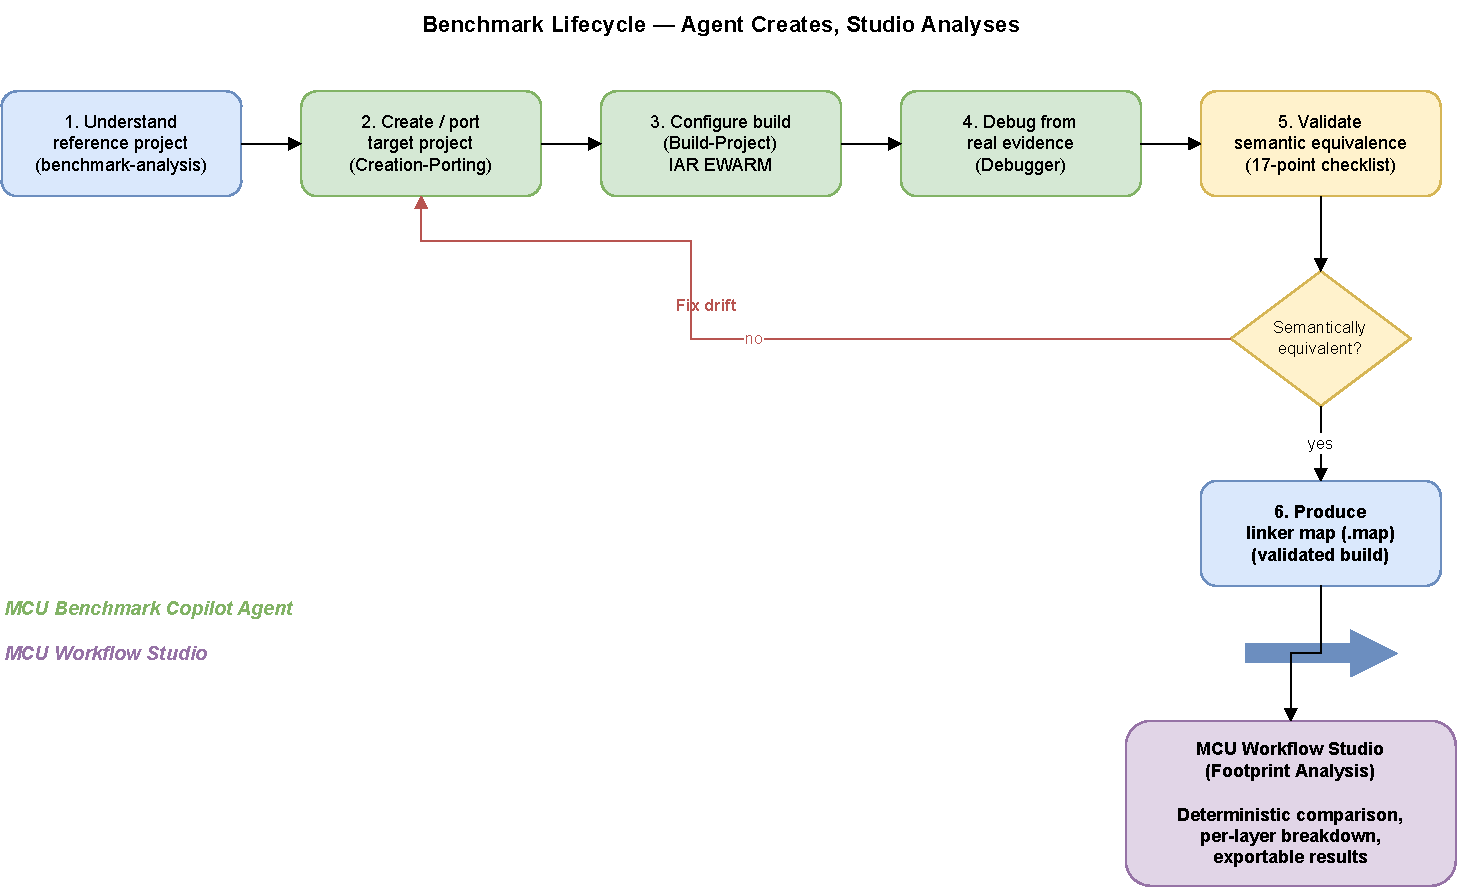
\includegraphics[width=\textwidth]{Figures/benchmark-agent/workflow.pdf}
\caption{End-to-end benchmark lifecycle. The MCU Benchmark Copilot Agent handles steps~1
through~11 autonomously (with a hardware gate at step~9); once semantic equivalence is
confirmed, the validated linker map is handed to MCU Workflow Studio for footprint analysis.}
\label{fig:agent-workflow}
\end{figure}

Figure~\ref{fig:agent-sequence} presents the same campaign as a UML sequence diagram,
showing the actual participant delegation, message flow, the hardware approval gate, and
artifact emission at each step.

\begin{figure}[H]
\centering
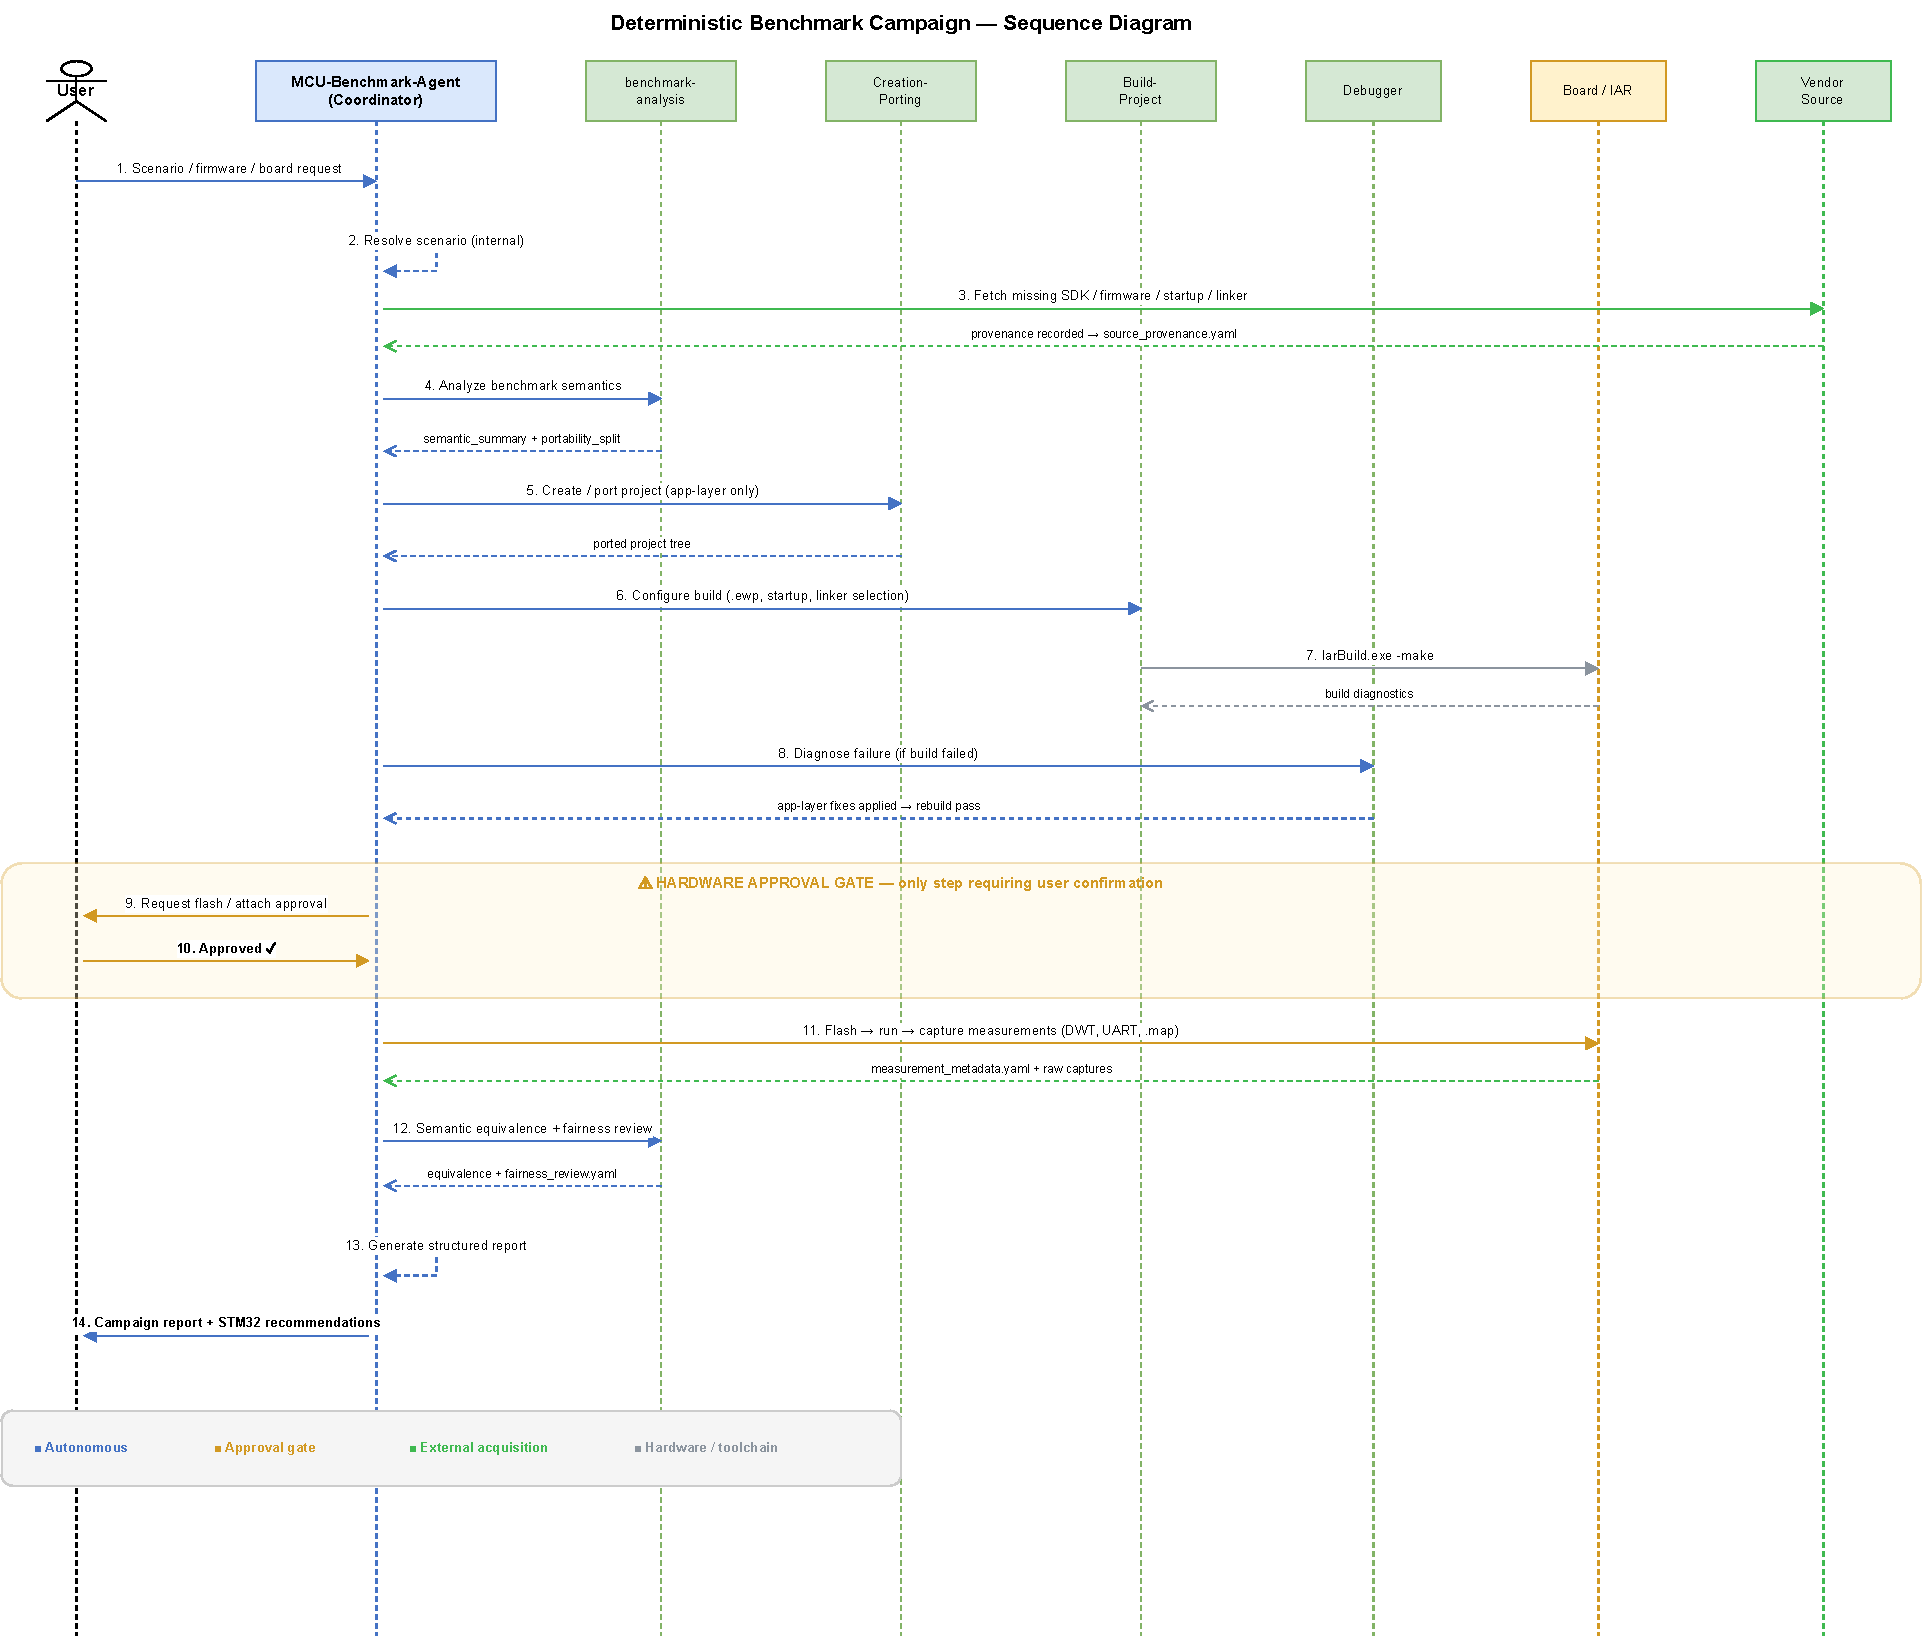
\includegraphics[width=\textwidth]{Figures/benchmark-agent/sequence.pdf}
\caption{UML sequence diagram of a deterministic benchmark campaign. The coordinator
delegates to specialist agents (benchmark-analysis, Creation-Porting, Build-Project,
Debugger) and interacts with external actors (Vendor Source, Board/IAR). The hardware
approval gate (steps~9--10, highlighted) is the only point requiring user confirmation;
all other steps execute autonomously.}
\label{fig:agent-sequence}
\end{figure}

This separation keeps each tool focused. The agent does not attempt footprint analysis, and
the studio does not attempt code generation or debugging. Together, they cover the full
lifecycle of a cross-vendor benchmark: resolve, acquire, create, build, debug, validate,
measure, then analyse.

\section{IAR template resolution}
\label{sec:agent-iar-templates}

Before creating any benchmark project, the system must resolve the correct IAR project
template for the target board. We designed a deterministic four-step resolution algorithm
encoded in the \emph{iar-template-resolution} skill:

\begin{enumerate}
\item \textbf{Exact board match} --- search the template registry (\texttt{iar\_templates.yaml}) for an entry whose \texttt{board\_id} matches the target exactly.
\item \textbf{Family fallback} --- if no exact match, search for a family-level fallback template and adjust device, startup, and linker for the specific MCU.
\item \textbf{Board-type fallback} --- if no family match, select the closest template matching the board type and vendor with explicitly downgraded confidence.
\item \textbf{Unresolved} --- if no suitable template exists, document the gap and report to the user rather than fabricating a template.
\end{enumerate}

When a template is identified but not yet materialised locally, the
\texttt{acquire\_iar\_template.ps1} script fetches it from official vendor GitHub
repositories or SDK packages, records provenance, and verifies the file inventory. The
materialised template then serves as the read-only project baseline into which benchmark
application code is integrated through designated integration points.

\section{Source acquisition policy}
\label{sec:agent-acquisition}

When materials are missing, the agent acquires them autonomously using a strict preference
order:

\begin{enumerate}
\item Workspace files already present.
\item Local SDK content (IAR device/config directories, installed CMSIS packs).
\item Official vendor GitHub repositories (tagged releases preferred).
\item Official vendor websites, SDK packages, CMSIS Pack Index.
\item Third-party mirrors --- only as a last resort, with an explicit risk note.
\end{enumerate}

For every acquired resource, the agent records: source URL, version or branch/tag/commit,
package name, and date of acquisition. This provenance chain ensures that any benchmark
result can be traced back to the exact firmware version used, satisfying the
reproducibility requirements of academic evaluation.

\section{Campaign artifact model}
\label{sec:agent-artifacts}

Each benchmark campaign persists its state in a structured dossier under
\texttt{.github/benchmark/campaigns/<campaign\_id>/}. Key artifacts include:

\begin{itemize}
\item \texttt{campaign\_manifest.yaml} --- campaign identity, platforms, and stage tracking.
\item \texttt{execution\_status.yaml} --- per-stage status with timestamps and blockers.
\item \texttt{source\_provenance.yaml} --- acquisition provenance for every resource used.
\item \texttt{scenario\_resolution.yaml} --- how partial input was resolved.
\item \texttt{fairness\_baseline.yaml} --- per-platform configuration baseline for fairness comparison.
\item \texttt{semantic\_equivalence.yaml} --- verification results per checklist item.
\item \texttt{fairness\_review.yaml} --- all fairness-sensitive differences identified.
\item \texttt{measurement\_metadata.yaml} --- metrics collected, methods, triggers, and confidence levels.
\end{itemize}

This artifact model makes every campaign auditable and reproducible. A reviewer can inspect
the dossier to understand exactly what was resolved, acquired, built, measured, and
concluded --- without re-running the campaign.

\section{Prompt-driven usage}
\label{sec:agent-prompts}

To lower the barrier to entry, the system ships ten pre-built prompt templates
(\texttt{.github/prompts/}) that encode common benchmark tasks. The user selects a prompt
from the Copilot chat picker and fills in minimal parameters (a board name, a scenario, or
a firmware package name); the agent handles everything else. Table~\ref{tab:agent-prompts}
lists the available prompts.

\begin{table}[H]
\centering
\caption{Pre-built prompt templates for common benchmark tasks.}
\label{tab:agent-prompts}
\begin{tabularx}{\textwidth}{c X}
\toprule
\textbf{\#} & \textbf{Purpose} \\
\midrule
01 & Autonomous benchmark from firmware name only --- agent resolves, acquires, builds, and measures. \\
02 & Port a benchmark to another board with fairness guarantee. \\
03 & Build, debug, and measure an existing project autonomously. \\
04 & Compare two boards fairly with semantic-equivalence check. \\
05 & Recommend STM32 improvements after a measured competitor gap. \\
06 & Create a new benchmark from a scenario description (no reference). \\
07 & Port STM32 reference to a competitor platform. \\
08 & Port competitor benchmark to STM32. \\
09 & Port between two non-ST vendors. \\
10 & Resolve and build from a firmware/SDK package name alone. \\
\bottomrule
\end{tabularx}
\end{table}

% TODO(screenshot): Replace placeholder with actual VS Code agent session screenshot
\begin{figure}[H]
\centering
\fbox{\parbox{0.9\textwidth}{\centering\vspace{4cm}\textbf{[PLACEHOLDER --- VS Code agent session screenshot]}\\Capture a VS~Code window showing the Copilot Chat panel with the MCU Benchmark\\Agent active during an autonomous campaign (showing structured output with\\provenance, semantic equivalence, and fairness review).\vspace{4cm}}}
\caption{An autonomous benchmark campaign in VS~Code: the MCU Benchmark Copilot Agent resolves the scenario, acquires firmware, builds, and reports semantic equivalence and fairness status.}
\label{fig:agent-session}
\end{figure}

\section{Implementation}
\label{sec:agent-implementation}

The entire agent system is implemented within a \texttt{.github/} directory, leveraging the
VS Code GitHub Copilot extensibility framework~\cite{github-copilot, vscode-agent-mode,
vscode-custom-agents}.
Agent and skill definitions use YAML frontmatter to declare metadata (name, description,
tool permissions) and Markdown bodies for behavioural instructions. The automation tools are
standalone PowerShell and Python scripts. Table~\ref{tab:agent-impl} summarises the file
structure.

\begin{table}[H]
\centering
\caption{File structure of the agent system.}
\label{tab:agent-impl}
\begin{tabularx}{\textwidth}{l X}
\toprule
\textbf{Path} & \textbf{Role} \\
\midrule
\texttt{.github/copilot-instructions.md} & Always-on rules inherited by every agent and skill. \\
\texttt{.github/agents/*.agent.md} & One file per specialist agent (4 files). \\
\texttt{.github/skills/*/SKILL.md} & One directory per skill, each containing a structured checklist (6 directories). \\
\texttt{.github/tools/*.ps1, *.py} & Twelve automation scripts for deterministic operations. \\
\texttt{.github/config/*.yaml} & Eight configuration registry files (boards, MCUs, vendors, toolchains, templates, sources, measurements, reporting). \\
\texttt{.github/prompts/*.prompt.md} & Ten pre-built prompt templates for common tasks. \\
\texttt{.github/templates/benchmark-dossier/} & Campaign artifact templates (YAML skeletons). \\
\texttt{.github/docs/} & Developer documentation (quickstart, porting guide, validation guide, naming conventions, etc.). \\
\texttt{.github/schemas/} & JSON/YAML schemas for artifact validation. \\
\bottomrule
\end{tabularx}
\end{table}

The implementation requires no external server, no API keys beyond the user's existing
GitHub Copilot subscription, and no deployment pipeline. Adding a new agent, skill, tool,
or board entry is a matter of creating a file and restarting the Copilot Chat session. This
minimal footprint was deliberate: the system should be as easy to maintain and
version-control as the benchmark source code itself.

\section{Integration with the benchmarking workflow}
\label{sec:agent-integration}

The agent system occupies a precise position in the benchmarking pipeline. It sits
\emph{before} MCU Workflow Studio in the workflow: the agent resolves the scenario, acquires
materials, creates and validates the target project, ensures it compiles under IAR EWARM,
confirms that its runtime behaviour matches the reference, and extracts measurements. Only
then does the build's linker map become an input to MCU Workflow Studio for footprint
analysis. The relationship is strictly sequential and complementary --- the agent is
responsible for \emph{producing and validating} correct builds, and the studio is
responsible for \emph{measuring and comparing} them.

\section{Engineering value and limitations}
\label{sec:agent-value}

The agent system's primary value is \emph{autonomous methodology enforcement at scale}. By
encoding the semantic-equivalence checklist, the fairness checklist, the evidence-driven
validation policy, the baseline immutability rule, and the provenance tracking requirement
directly into the tool's behaviour, we ensure that every benchmark campaign follows the
same discipline regardless of which vendor is targeted or how many campaigns run in
parallel.

In practical terms, the agent reduces the time to produce a correct, validated target
project from several hours of manual porting and debugging to an autonomous session
requiring human intervention only at the hardware-programming gate. The deterministic
workflow, the configuration registry, and the campaign artifact model make every result
auditable and reproducible.

The structured output contracts --- each agent returns objective, scenario resolution,
actions executed, semantic equivalence status, fairness status, key findings, unresolved
unknowns, and next action --- make the work transparent and reviewable without re-executing
the campaign.

We acknowledge several limitations. The system depends on the quality of the underlying
language model; while the always-on rules and the configuration registry constrain its
behaviour, they cannot prevent all model errors, particularly for vendor APIs that are
poorly represented in the model's training data. The tool supports IAR EWARM~9.60.3 as the
primary toolchain; extending it to other compilers (GCC, Keil) would require additional
Build-Project configurations and toolchain registry entries. The evidence-driven validation
policy means the system halts at the hardware gate --- it cannot flash a board without
explicit approval. This is by design: in embedded benchmarking, the hardware is the ground
truth, and no amount of static reasoning can substitute for it.

\section*{Conclusion}

We designed and built the MCU Benchmark Copilot Agent as an autonomous campaign coordinator
that fills the engineering gap between defining a benchmark and having a validated,
measured, and fairly compared result. Its four specialist agents cover the full lifecycle
from scenario resolution to measurement extraction; its six reusable skills encode our
methodology as structured checklists; its twelve automation tools provide deterministic
execution; and its configuration registry eliminates hallucination for known hardware facts.
The always-on rules enforce semantic equivalence, benchmark fairness, baseline immutability,
provenance tracking, and evidence-driven validation at every step.

Together with MCU Workflow Studio, the agent forms a complete autonomous toolchain for
reproducible, explainable cross-vendor firmware benchmarking: the agent resolves, acquires,
creates, builds, debugs, validates, and measures; the studio analyses the resulting
footprint. The system supports eight MCU vendors, six workflow directions, and ten
pre-built prompt templates --- making it scalable to the full breadth of the STM32Cube
competitive analysis campaign.

\pagebreak